%La figura~\ref*{fig:primerafigura} muestra algunas líneas de la imagen-ejemplo.
\documentclass{book}
\usepackage[spanish,mexico]{babel}
\usepackage[utf8]{inputenc}
\usepackage{graphicx}
\usepackage{listings}
\usepackage{showexpl}
\usepackage{booktabs}
\usepackage{hyperref}
\usepackage{xr}

\lstset{
    inputencoding=utf8,
    extendedchars = true,
    basicstyle=\ttfamily\small,
    keywordstyle=,
    stringstyle=,
    commentstyle=,
    breaklines=true,
    numbers=none,
    rframe=
}

\newfloat{codigo}{H}{loc}[chapter]
\floatname{codigo}{Código}

\begin{document}
\chapter*{Entornos flotantes}\label{ch:entornos flotantes}
Los entornos flotantes entornos flotantes en LaTeX permiten incluir elementos como tablas y figuras que se ajustan automáticamente dentro del documento, respetando el diseño y facilitando las referencias cruzadas.

Por omisión \LaTeX\ ofrece dos tipos de entornos flotantes, \texttt{figure} y \texttt{table}. Es posible controlar su posición en el documento usando los parámetros `h`, `t`, `b`, `p`, entre otros.

\begin{table}[h!]
    \centering
    \begin{tabular}{c|c|l}
         \hline
         Parámetro & Significado & Descripción \\ \hline
         h & here & Aparece donde se invoca el comando. \\ \hline
         t & top & Se coloca al inicio de la página. \\ \hline
         b & bottom & Se coloca al final de la página. \\ \hline
         p & page of floats & Se envía a una página dedicada a flotantes. \\ \hline
         ! & override & Fuerza la posición especificada. \\ \hline
    \end{tabular}
    \caption{Parámetros para controlar la posición de los flotantes.}
    \label{tabla:parametros_posicion}
\end{table}

\section{Entornos Básicos}
\subsection{Figuras (\texttt{figure})}
El entorno \texttt{figure} se utiliza para insertar imágenes o gráficas. Las figuras pueden ajustarse en tamaño usando los parámetros \texttt{'width'}, \texttt{'height'} o \texttt{'scale'}. Así como cenrtar la imagen usando \verb|\centering|.

Para crear un índice con todas las figuras del documento, se utiliza \verb|\listoffigures|.\\

\subsubsection*{Sintaxis:}
\begin{codigo}
\begin{center}
    \begin{lstlisting}[language=TeX]
        \begin{figure}[parametros de posicion]
          \includegraphics[parametros de tamano]{imagen}
          \caption{titulo de la imagen}
          \label{etiqueta}              
        \end{figure}
    \end{lstlisting}
\end{center}
\caption{Sintaxis del entorno \texttt{figure}}
\label{sintaxis:figure}
\end{codigo}


\subsubsection*{Ejemplos:}
\begin{itemize}
    \item Si no se especifica que la imagen debe ir centrada, \LaTeX 
 la coloca a la izquierda del documento.
\begin{codigo}    
\begin{LTXexample}[numbers=none]
        \begin{figure}[h!]
          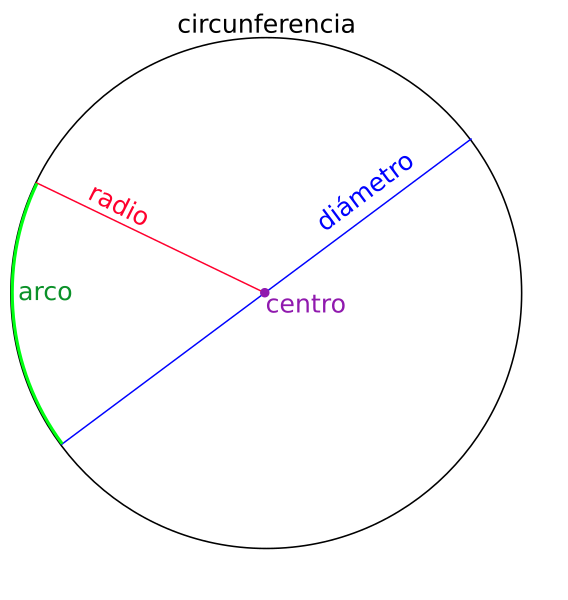
\includegraphics[width=2cm]{imagen-ejemplo}
          \caption{Circunferencia}
          \label{ej_fig_iz}              
        \end{figure}
\end{LTXexample}
\label{ejemplo:figure_sin centrar}
\end{codigo}

    \item Modifica el tamaño de la imagen utilizando \texttt{width} y \texttt{height}.
    \begin{codigo}
    \begin{LTXexample}[numbers=none]
        \begin{figure}[h!]
          \centering
          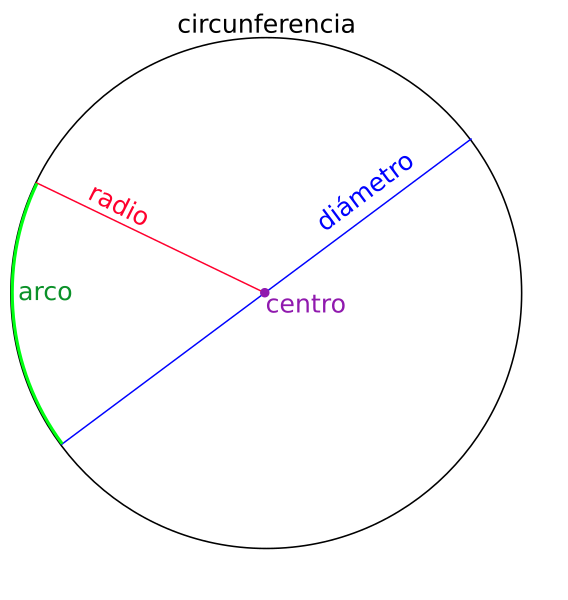
\includegraphics[width=2cm, height=1cm]{imagen-ejemplo}
          \caption{Título}
          \label{etiqueta}              
        \end{figure}
    \end{LTXexample}
    \label{ejemplo:figure_ancho y alto}
    \end{codigo}

    \item Imagen modificada usando \texttt{scale}
    \begin{codigo}
    \begin{LTXexample}[numbers=none]
        \begin{figure}[htp]
          \centering
          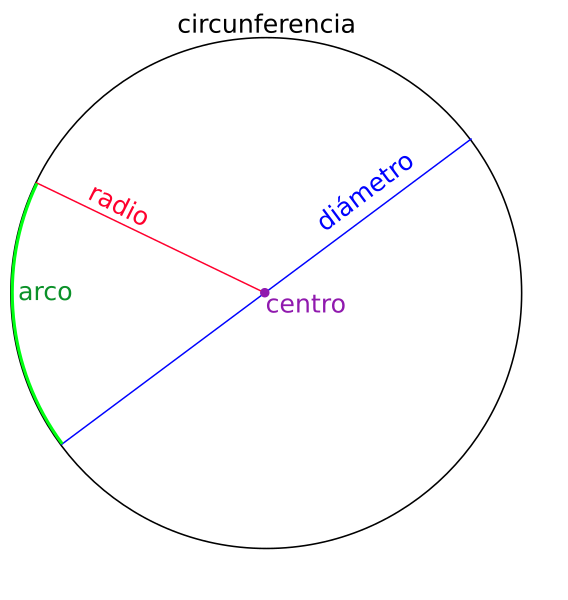
\includegraphics[scale=0.2]{imagen-ejemplo}
          \caption[loftitle]{title}
          \label{etiqueta}              
        \end{figure}
    \end{LTXexample}
    \label{ejemplo:figure_escala}
    \end{codigo}

\end{itemize}

\subsection{Table (\texttt{table})}\label{table}
Las tablas se usan para estructurar datos en filas y columnas. Se pueden personalizar ajustando alineaciones y bordes.

Para crear un índice con todas las figuras del documento, se utiliza \verb|\listoftables|.\\

\begin{table}[h]
    \centering
    \begin{tabular}{c|c|l}
        \hline
        Parámetro & Significado & Descripción\\
        \hline
        l & left & Alinea el texto a la izquierda de la celda \\
        \hline
        c & center & Centra el texto de la celda\\
        \hline
        r & right & Alinea el texto a la derecha de la celda\\
        \hline
    \end{tabular}
    \caption{Parámetros para controlar la posición del texto en una tabla.}
    \label{tabla:parametros_tabla}
\end{table}

\subsubsection*{Sintaxis:}
\begin{codigo}
\begin{LTXexample}[numbers=none]
    \begin{table}[placement]
        \centering
        \begin{tabular}{|c|c|c|}
        \hline
        Columna 1 & Columna 2 & Columna 3 \\ \hline
        Dato 1 & Dato 2 & Dato 3 \\ \hline
    \end{tabular}
    \caption{Título de la tabla.}
    \label{unatabla}
    \end{table}
\end{LTXexample}
\label{sintaxis:table}
\end{codigo}

\subsubsection*{Ejemplos:}

\begin{itemize}
    \item Usando la imagen 
    \begin{codigo}
    \begin{LTXexample}[numbers=none]
        \begin{table}[h]
            \centering
            \begin{tabular}{lcrp{3cm}}
            \toprule
            Color & Forma & Posición & Nombre \\ \midrule
            Azul & Recta & Dentro & Diámetro\\ 
            Rojo & Recta & Dentro & Radio\\
            Verde & Curva & Sobre & Arco\\
            \bottomrule
            \end{tabular} 
        \caption{Título de la tabla.}
        \label{tabla:unatabla}
        \end{table}
    \end{LTXexample}
    \label{ejemplo:table}
    \end{codigo}

\end{itemize}

\section{Buenas prácticas}
\begin{enumerate}
    \item Aunque  ambos entornos acceptan imágenes y texto, usa `figure` para imágenes y diagramas, y `table` para datos tabulados.
    \item Siempre incluye etiquetas (`\verb|\label|`) para facilitar las referencias cruzadas.
    \item Para controla con mayor precisión la posición de los flotantes utiliza el paquete \hyperref[ch:float]{\texttt{float}}.
\end{enumerate}


\end{document}
